\part{Forced-Oscillations}
\lecture{Forced Oscillations}{Forced-Oscillations}
\section{Forced Oscillations}

\title{Ordinary Differential Equations}
\subtitle{Math 232 - Forced Oscillations}
\date{22 October 2012}

\begin{frame}
  \titlepage
\end{frame}

\begin{frame}
  \frametitle{Outline}
  \tableofcontents[pausesection,hideothersubsections]
\end{frame}


\subsection{Forced Oscillations}


\begin{frame}
  \frametitle{Forced Oscillations}

  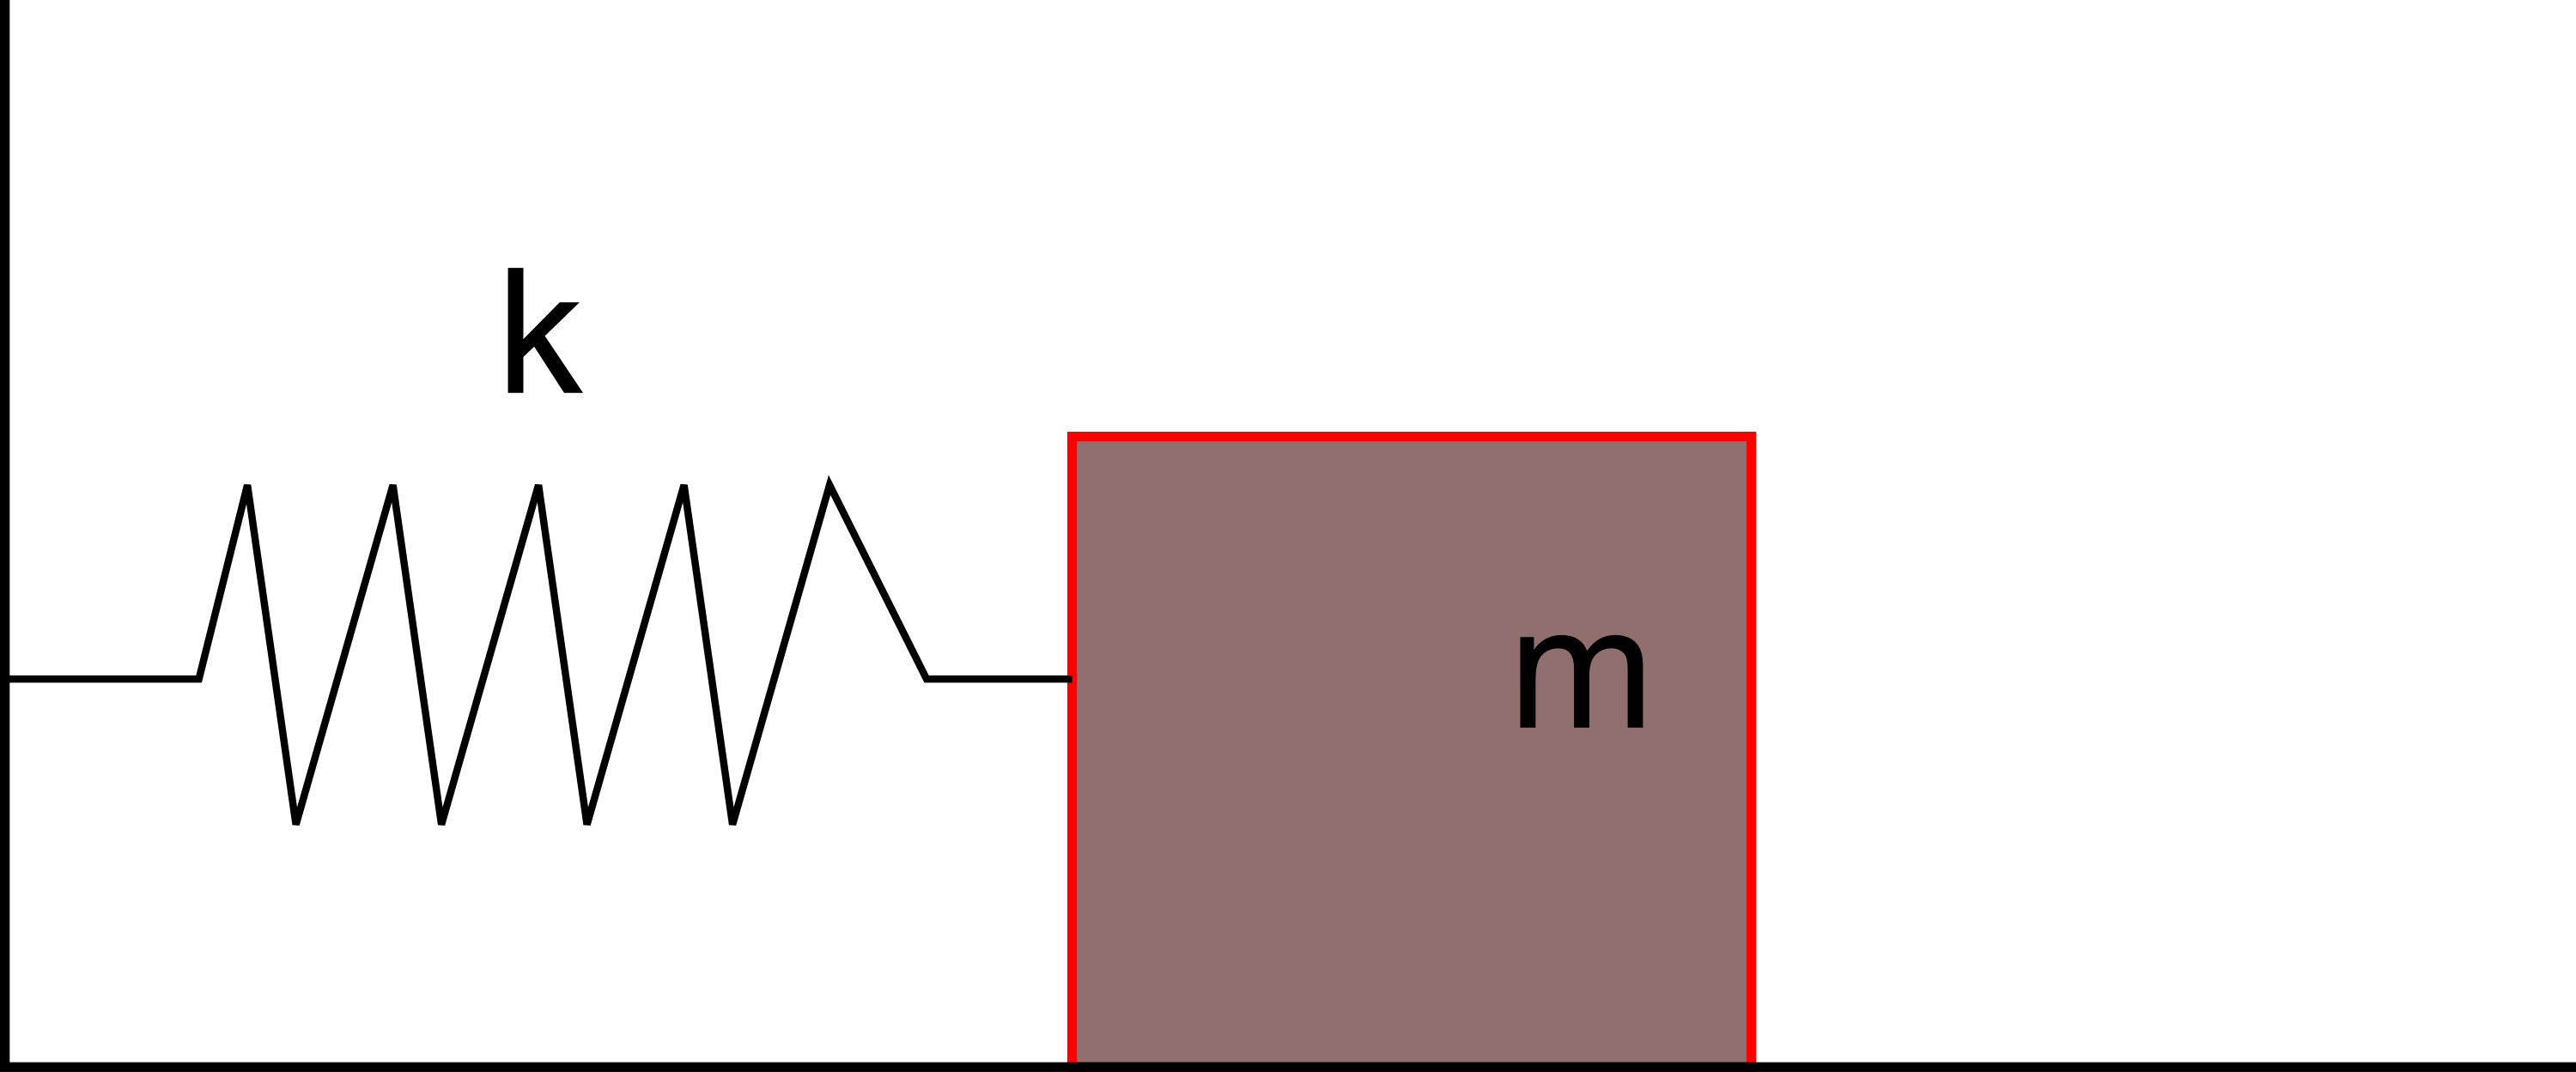
\includegraphics[width=6cm]{img/springMassStatic}

  Section 4.1 - Redux: The governing equation for a mass/spring system
  is
  \begin{eqnarray*}
    mx'' + bx'+kx & = & f(t).
  \end{eqnarray*}

  The constants $m$, $b$, and $k$ are all non-negative.

  The function $f(t)$ is called the \textit{forcing function}.

  This is a \underline{\textit{conceptual model}} for many physical systems.

\end{frame}


\begin{frame}
  \frametitle{Special Case}

  Suppose that we have a periodic forcing:
  \begin{eqnarray*}
    f(t) & = & F_0 \cos(\omega t), \\
    x(0) & = & 0, \\
    x'(0) & = & 0.
  \end{eqnarray*}

  Suppose that there is no friction, $b=0$,
  \begin{eqnarray*}
    m x'' + kx & = & F_0 \cos(\omega t).
  \end{eqnarray*}

  This is an idealized system used to gain insight into real physical
  systems. It allows us to ask \textit{``what if....?''}

\end{frame}


\begin{frame}
  \frametitle{Homogeneous and Particular Solution}

  \begin{eqnarray*}
    x_h & = & C_1 \cos\lp\sqrt{\frac{k}{m}}t\rp + C_2 \sin\lp\sqrt{\frac{k}{m}}t\rp.
  \end{eqnarray*}

  Assume that $\omega \neq \sqrt{\frac{k}{m}}$, then the particular
  solution is
  \begin{eqnarray*}
    x_p & = & \frac{F_0}{m\lp\frac{k}{m}-\omega^2\rp} \cos(\omega t).
  \end{eqnarray*}

  \uncover<2->{You should be able to show this on your own using ideas we have already covered in class.}

\end{frame}


\begin{frame}
  \frametitle{Solve for the Constants}

  \begin{eqnarray*}
    x & = & C_1 \cos\lp\sqrt{\frac{k}{m}}t\rp + C_2 \sin\lp\sqrt{\frac{k}{m}}t\rp+ 
           \frac{F_0}{m\lp\frac{k}{m}-\omega^2\rp} \cos(\omega t).
  \end{eqnarray*}

  The initial conditions yield
  \begin{eqnarray*}
    x(0) & = & C_1 + \frac{F_0}{m\lp\frac{k}{m}-\omega^2\rp} \\
    \Rightarrow C_1 & = & \frac{-F_0}{m\lp\frac{k}{m}-\omega^2\rp}
  \end{eqnarray*}

\end{frame}


\begin{frame}
  \frametitle{Satisfy the Velocity}

  \begin{eqnarray*}
    x' & = & - C_1 \sqrt{\frac{k}{m}} \sin\lp\sqrt{\frac{k}{m}}t\rp + C_2 \sqrt{\frac{k}{m}} \cos\lp\sqrt{\frac{k}{m}}t\rp \\ 
    & & - \frac{\omega F_0}{m\lp\frac{k}{m}-\omega^2\rp} \sin(\omega t), \\
    \Rightarrow C_2 & = & 0.
  \end{eqnarray*}

  \uncover<2->
  {
    The solution is 
    \redText{
      \begin{eqnarray*}
        x & = & \frac{-F_0}{m\lp\frac{k}{m}-\omega^2\rp} \cos\lp\sqrt{\frac{k}{m}}t\rp 
        + \frac{F_0}{m\lp\frac{k}{m}-\omega^2\rp} \cos(\omega t).
      \end{eqnarray*}
    }
  }


\end{frame}


\begin{frame}
  \frametitle{Obvious Trigonometric Identity}

  As we \textbf{all} know
  \begin{eqnarray*}
    \cos(u) - \cos(v) & = & -2 \sin\lp\frac{u-v}{2}\rp \sin\lp\frac{u+v}{2}\rp.
  \end{eqnarray*}

  Our solution can be written in the form
  \begin{eqnarray*}
    x(t) & = & \frac{-F_0}{m\lp\frac{k}{m}-\omega^2\rp} \sin\lp\lp\omega-\sqrt{\frac{k}{m}}\rp t\rp
                                                        \sin\lp\lp\omega+\sqrt{\frac{k}{m}}\rp t\rp
  \end{eqnarray*}

  Plots of the function are given on pages 262-267 in your book.

\end{frame}

\subsection{Example}

\iftoggle{clicker}{%
\begin{frame}
  \frametitle{Clicker Quiz}

      \ifnum\value{clickerQuiz}=1{%

        \vfill

        Determine the homogeneous solution to the differential equation
        \begin{eqnarray*}
          2 x'' + 10 x & = & 3 \cos(2t)
        \end{eqnarray*}


        \vfill

        \begin{tabular}{ll}
          A: & $x=C_1\cos(5t) + C_2\sin(5t)$ \\
          B: & $x=C_1\cos(\sqrt{5}t) + C_2\sin(\sqrt{5}t)$ \\
          C: & $x=C_1e^{5t} + C_2 t e^{5t}$ \\
          D: & $x=C_1e^{\sqrt{5t}} + C_2 t e^{\sqrt{5}t}$ \\
        \end{tabular}


        \vfill

      }\fi

      \ifnum\value{clickerQuiz}=2{%

        \vfill

        Determine the homogeneous solution to the differential equation
        \begin{eqnarray*}
          2 x'' + 10 x & = & 3 \cos(2t)
        \end{eqnarray*}


        \vfill

        \begin{tabular}{ll}
          A: & $x=C_1e^{5t} + C_2 t e^{5t}$ \\
          B: & $x=C_1e^{\sqrt{5t}} + C_2 t e^{\sqrt{5}t}$ \\
          C: & $x=C_1\cos(5t) + C_2\sin(5t)$ \\
          D: & $x=C_1\cos(\sqrt{5}t) + C_2\sin(\sqrt{5}t)$ \\
        \end{tabular}


        \vfill

     }\fi
   
     \ifnum\value{clickerQuiz}=3{%
         Determine the homogeneous solution to the differential equation
        \begin{eqnarray*}
          2 x'' + 10 x & = & 3 \cos(2t)
        \end{eqnarray*}


        \vfill

        \begin{tabular}{ll}
          A: & $x=C_1e^{5t} + C_2 t e^{5t}$ \\
          B: & $x=C_1e^{\sqrt{5t}} + C_2 t e^{\sqrt{5}t}$ \\
          C: & $x=C_1\cos(5t) + C_2\sin(5t)$ \\
          D: & $x=C_1\cos(\sqrt{5}t) + C_2\sin(\sqrt{5}t)$ \\
        \end{tabular}

        \vfill

    }\fi
  

\end{frame}
}


\begin{frame}                   
  \frametitle{The problem}      
                                
  A two kilogram mass is attached to a spring with constant ten N/m on
  a horizontal table. The mass is driven with a periodic force of
  \begin{eqnarray*}
    f(t) & = & 3 \cos(2t).
  \end{eqnarray*}
  the system is started from rest at the equilibrium point.

  Governing equation:
  \begin{eqnarray*}
    2 x'' + 10 x & = & 3 \cos(2t)
  \end{eqnarray*}

\end{frame}


\begin{frame}
  \frametitle{Solution}

  \begin{eqnarray*}
    2 x'' + 10 x & = & 3 \cos(2t), \\
    x(0) & = & 0, \\
    x'(0) & = & 0.
  \end{eqnarray*}

  The solution is 
  \begin{eqnarray*}
<<<<<<< HEAD
    x(t) & = & -\frac{3}{2}\cos(\sqrt{5} t) + \frac{3}{2} \cos(2 t), \\
         & = & \frac{3}{2} \left[ -\cos(\sqrt{5} t) + \cos(2 t) \right], \\
=======
    x(t) & = & -\frac{3}{2}\cos(\sqrt{5} t) + \frac{3}{2} \sin( 2 t), \\
         & = & \frac{3}{2} \left[ -\cos(\sqrt{5} t) + \sin( 2 t) \right], \\
>>>>>>> 1950a389b6a672562187c68872747aefd80a516b
         \only<1>{%
           & = & 3 \sin\lp\frac{2-\sqrt{5}}{2}t\rp \sin\lp\frac{2+\sqrt{5}}{2} t\rp.\\
         }
         \only<2->{%
           & = & 3 \sin\lp\underbrace{\frac{2-\sqrt{5}}{2}}_{\mathrm{long~wave}}t\rp 
                   \sin\lp\underbrace{\frac{2+\sqrt{5}}{2}}_{\mathrm{short~wave}} t\rp.
         }
  \end{eqnarray*}

\end{frame}

\begin{frame}
  \frametitle{Plots}

  \only<1>{\centerline{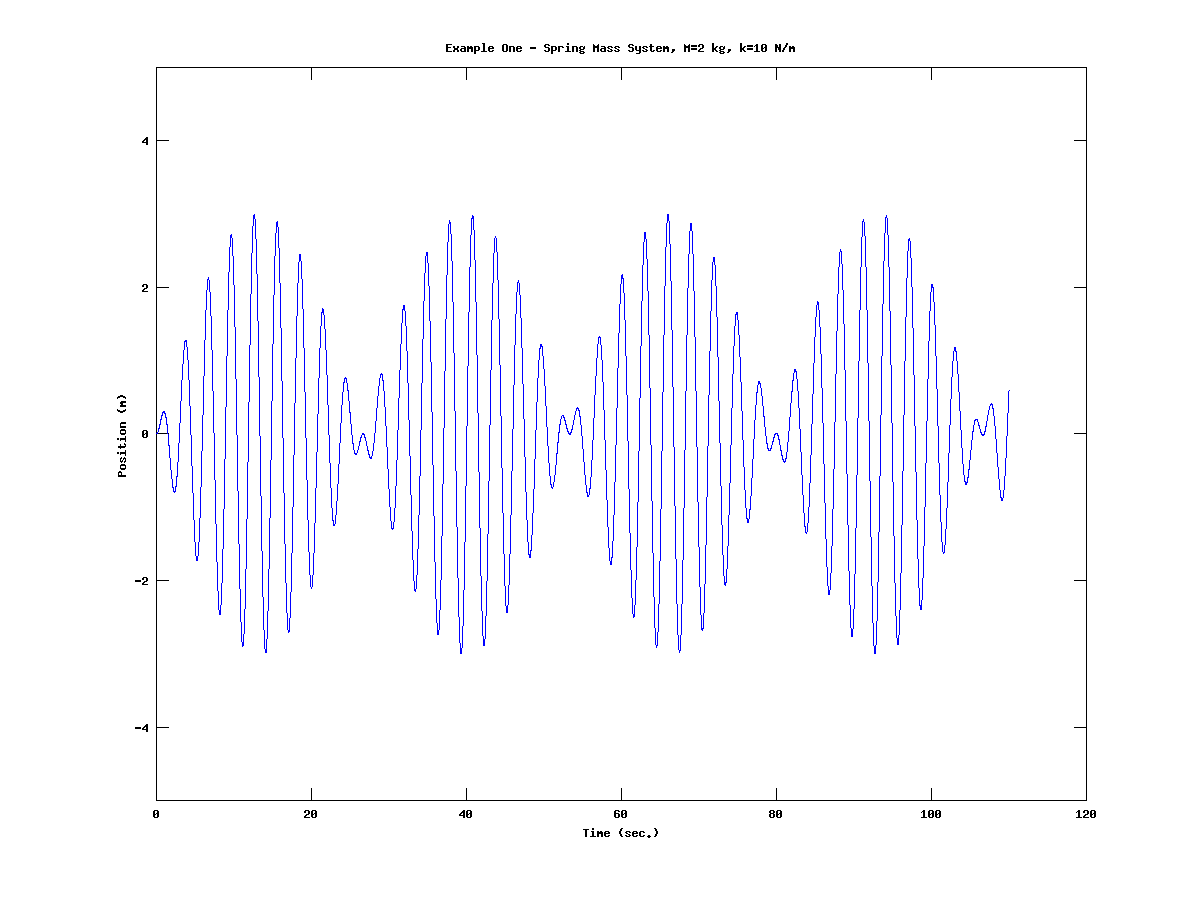
\includegraphics[width=11cm]{img/beats}}}
  \only<2>{\centerline{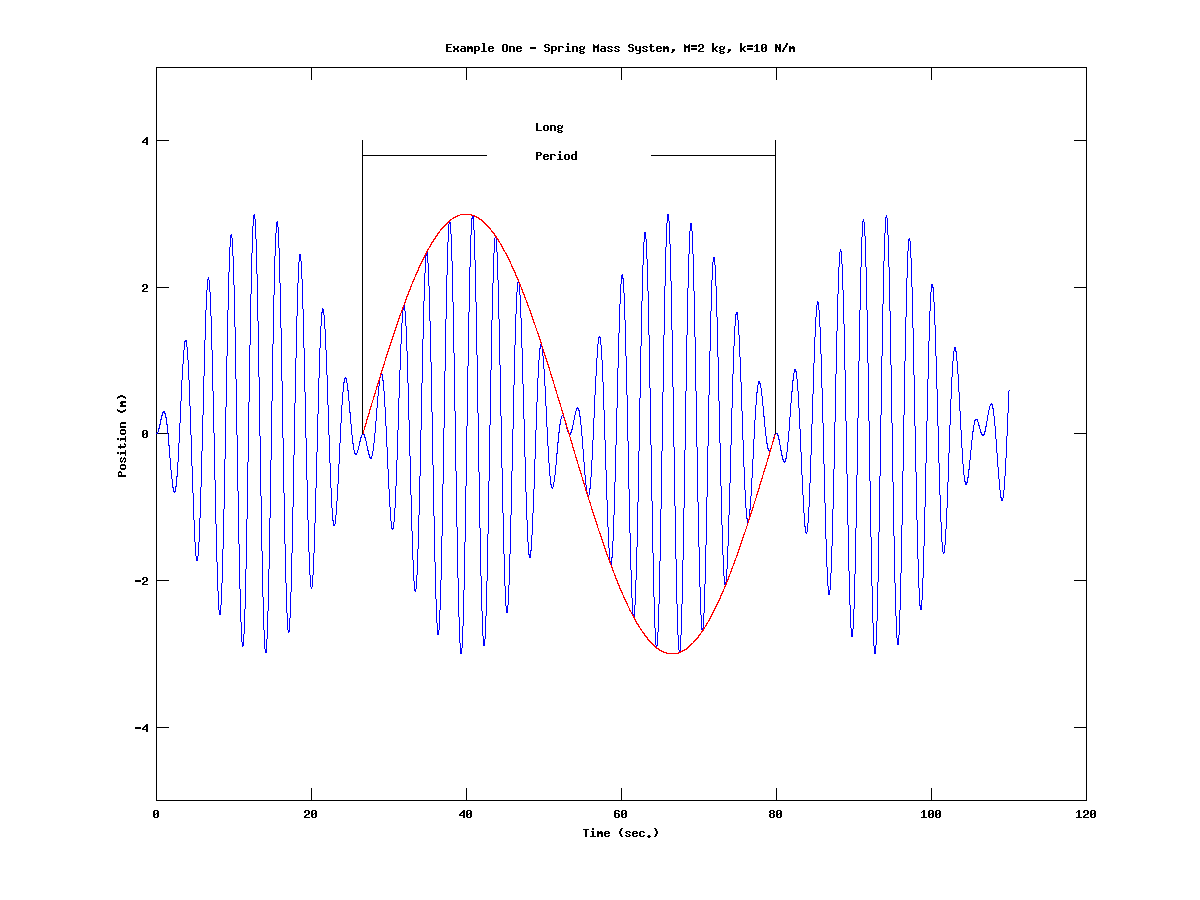
\includegraphics[width=11cm]{img/beatsLong}}}
  \only<3>{\centerline{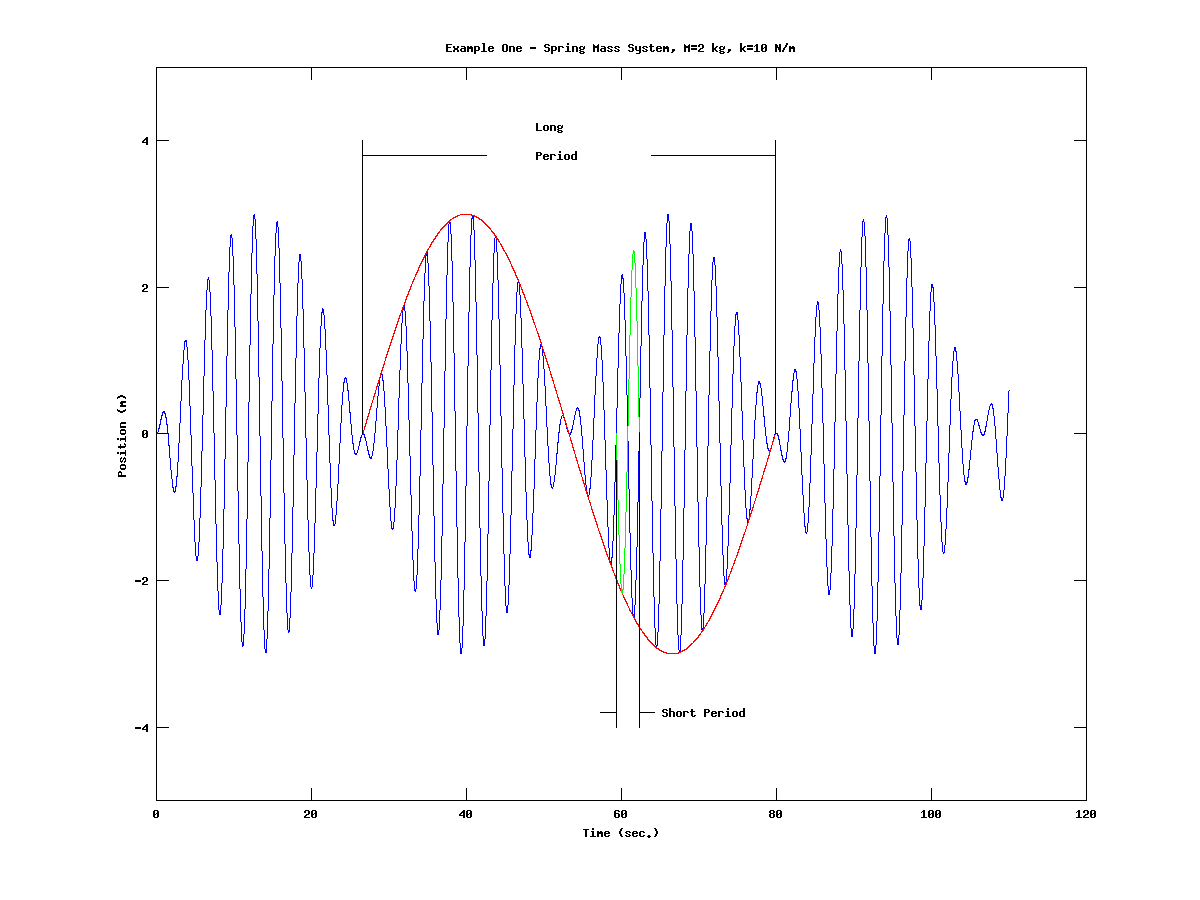
\includegraphics[width=11cm]{img/beatsShort}}}


\end{frame}



\begin{frame}
  \frametitle{The problem}      
                                
  A two kilogram mass is attached to a spring with constant ten N/m on
  a horizontal table. The mass is driven with a periodic force of
  \begin{eqnarray*}
    f(t) & = & 3 \cos(\sqrt{5} t).
  \end{eqnarray*}
  the system is started from rest at the equilibrium point.

  Governing equation:
  \begin{eqnarray*}
    2 x'' + 10 x & = & 3 \cos(\sqrt{5} t)
  \end{eqnarray*}

\end{frame}


\begin{frame}
  \frametitle{Solution}

  \begin{eqnarray*}
    2 x'' + 10 x & = & 3 \cos(\sqrt{5} t), \\
    x(0) & = & 0, \\
    x'(0) & = & 0.
  \end{eqnarray*}

  The homogeneous solution is 
  \begin{eqnarray*}
    x_h & = & C_1 \cos(\sqrt{5} t) + C_2 \sin(\sqrt{5} t).
  \end{eqnarray*}

  \only<2->
  {
    Guess a particular solution,
    \begin{eqnarray*}
      x_p & = & A t \cos(\sqrt{5} t) + B t \sin(\sqrt{5} t).
    \end{eqnarray*}
  }

\end{frame}

\begin{frame}
  \frametitle{The Solution}

  \begin{eqnarray*}
    x(t) & = & C_1 \cos(\sqrt{5}t) + C_2\sin(\sqrt{5} t) + \frac{3}{4\sqrt{5}} t \sin(\sqrt{5}t), \\
         & = & \frac{3}{4\sqrt{5}} t \sin(\sqrt{5}t).
  \end{eqnarray*}

  \only<2>{\centerline{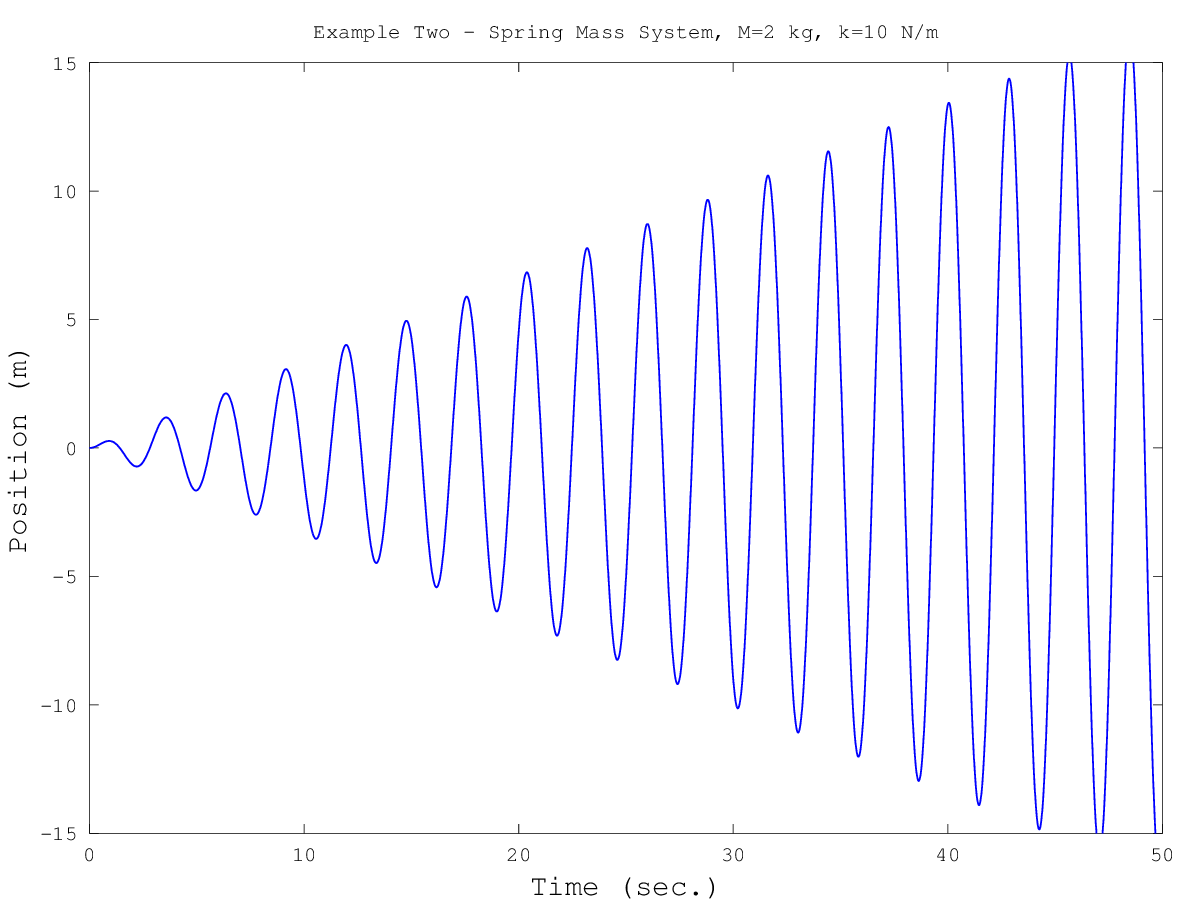
\includegraphics[width=5cm]{img/resonance}}}
  \only<3>{\centerline{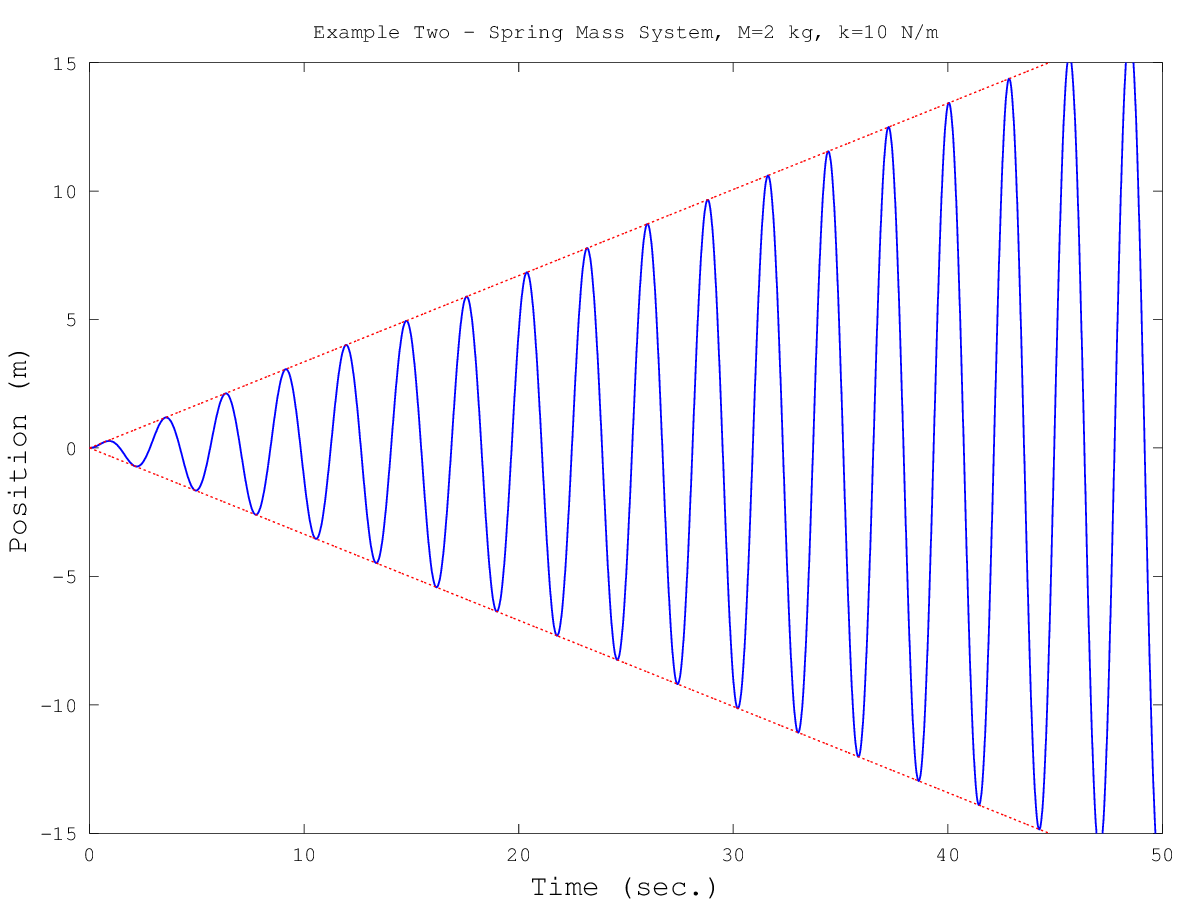
\includegraphics[width=5cm]{img/resonanceBounds}}}

\end{frame}


% LocalWords:  Clarkson pausesection hideothersubsections
